\renewcommand{\theequation}{\theenumi}
\begin{enumerate}[label=\arabic*.,ref=\thesubsection.\theenumi]
\item The equation of a circle is 
\begin{align}
\label{eq:circ_norm}
\norm{\vec{x}-\vec{c}} = r
\end{align}
%
where $\vec{c}$ is the centre and $r$ is the radius.
\item By expanding \eqref{eq:circ_norm}, the equation of a circle can also be expressed as
%
\numberwithin{equation}{enumi}
\begin{align}
\label{eq:circ_quad}
\norm{\vec{x}-\vec{c}}^2 = r^2&
\\
\implies \vec{x}^T\vec{x}-2\vec{c}^T\vec{x} + \vec{c}^T\vec{c}-r^2 = 0
\end{align}
\item The direction vector of {\em normal to the circle}  in \eqref{eq:circ_quad} at point $\vec{p}$ is
\begin{align}
\label{eq:circ_normal}
\vec{n} = k\brak{\vec{p}-\vec{c}},
\end{align}
%
where $k$ is a constant.
\item Find the equation of a circle that passes through the points $\vec{A},\vec{B},\vec{C}$.
\\
\solution From \eqref{eq:circ_quad},
\begin{align}
%\label{eq:circ_quad}
\norm{\vec{A}-\vec{c}}^2 = \norm{\vec{B}-\vec{c}}^2 = \norm{\vec{C}-\vec{c}}^2 &= r^2
\\
\implies \norm{\vec{A}-\vec{c}}^2 - \norm{\vec{B}-\vec{c}}^2 &=0
\end{align}
which can be simplified to obtain
\begin{align}
\brak{\vec{A}-\vec{B}}^T\vec{c}=\frac{\norm{\vec{A}}^2 - \norm{\vec{B}}^2}{2}& \quad \text{and}
\\
\brak{\vec{A}-\vec{C}}^T\vec{c}=\frac{\norm{\vec{A}}^2 - \norm{\vec{C}}^2}{2}& 
\end{align}
%
Solving the two yields $\vec{c}$, which can then be used to obtain $r$.
\item Let $\vec{A},\vec{B}$ and $\vec{C}$ be three points on the circle and 
$D$ be a point on $BC$ such that
$OD \perp BC$ as in Fig. \ref{fig:ccircle}.  Show that 
\begin{align}
\vec{D}=\frac{\vec{B}+\vec{C}}{2}
\end{align}
%
\begin{figure}[!ht]
	\begin{center}
		
		%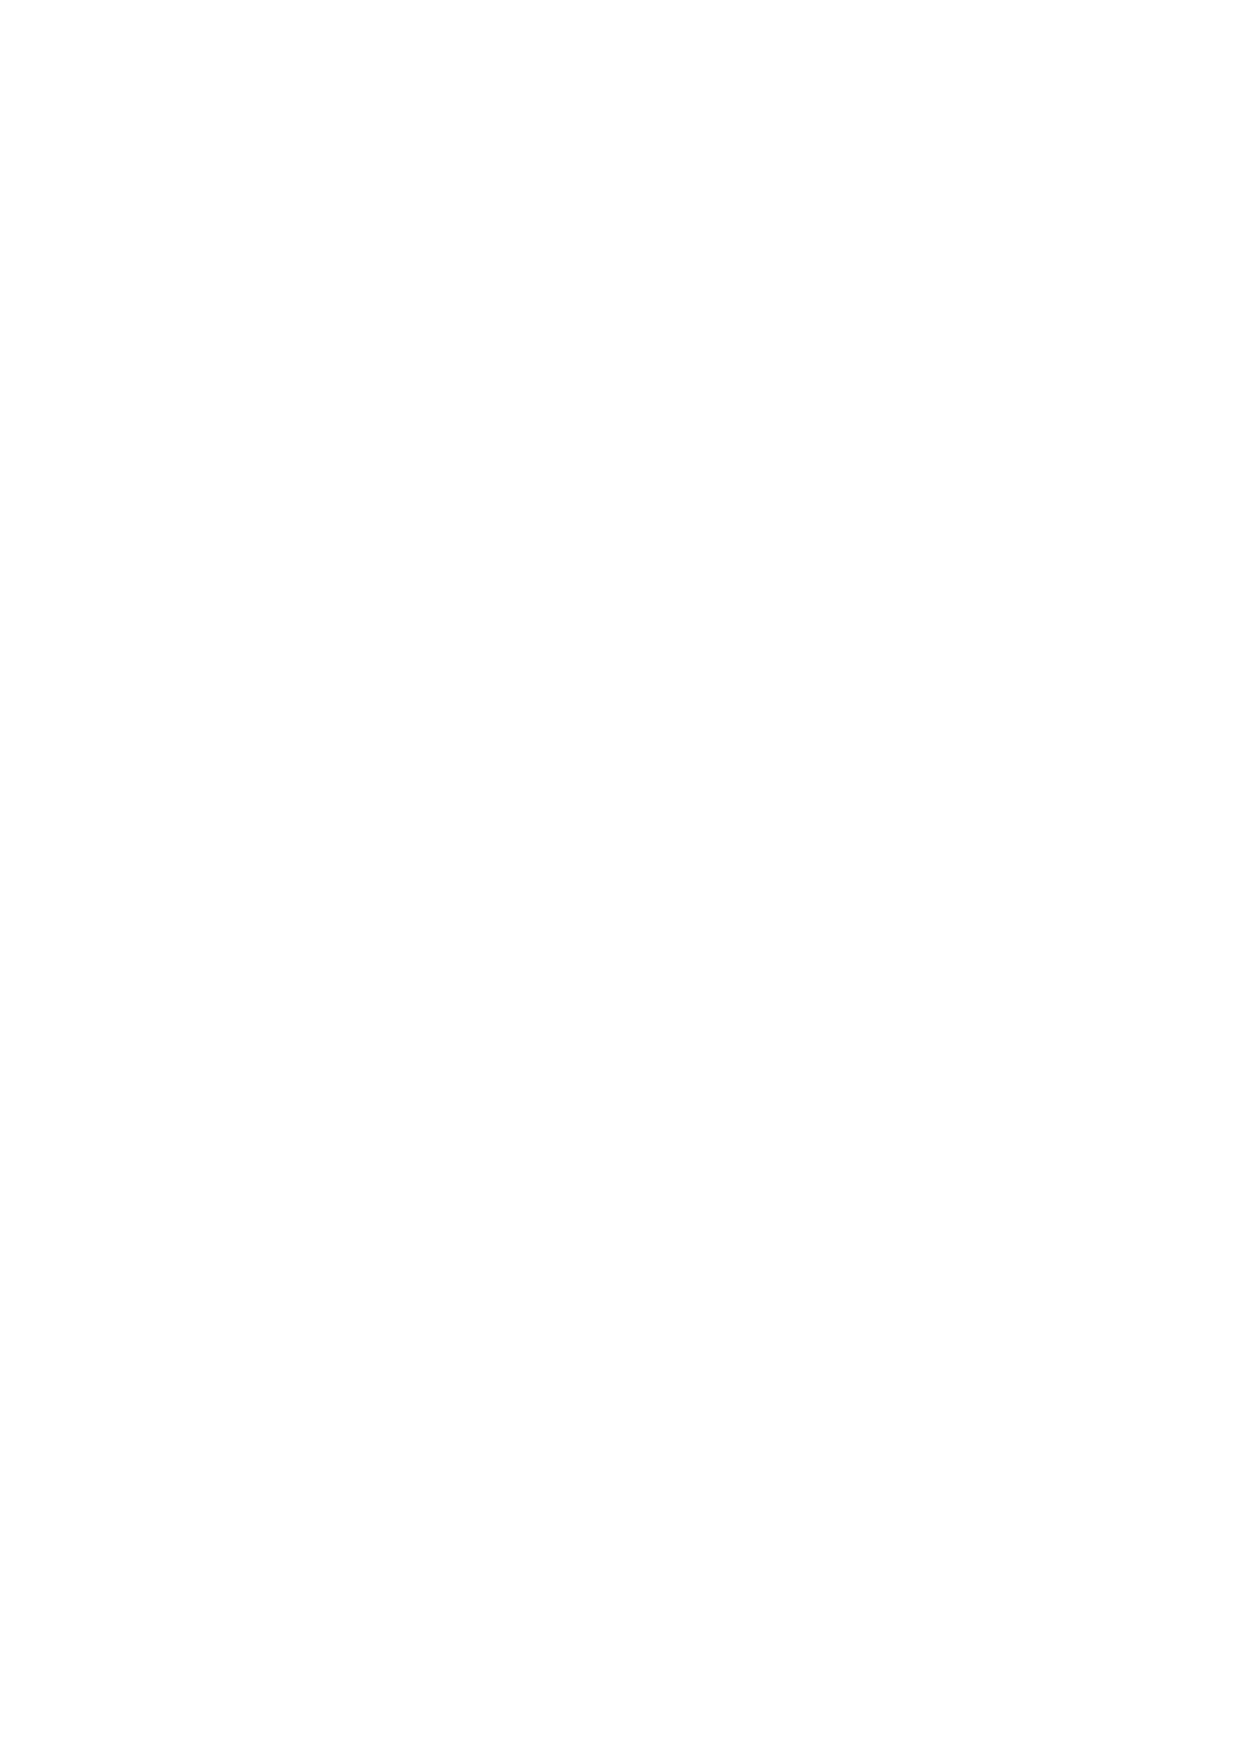
\includegraphics[width=\columnwidth]{./figs/ch3_angle_bisector}
		%\vspace*{-10cm}
		\resizebox{\columnwidth}{!}{\input{./figs/ccircle.tex}}
	\end{center}
	\caption{Circumcircle.}
	\label{fig:ccircle}	
\end{figure}


\solution From \eqref{eq:circ_norm}
\begin{align}
\norm{\vec{B}-\vec{O}}^2=\norm{\vec{C}-\vec{O}}^2=r^2
\\
 \implies \brak{\vec{B}-\vec{O}}^T\brak{\vec{B}-\vec{O}} = 
\brak{\vec{C}-\vec{O}}^T\brak{\vec{C}-\vec{O}} 
\\
 \implies \brak{\vec{B}-\vec{C}}^T\brak{\frac{\vec{B}+\vec{C}}{2} - 
\vec{O}}  = 0
\label{eq:circle_mid}
\end{align}
after simplification. Since $OD \perp BC$,
\begin{align}
\brak{\vec{B}-\vec{C}}^T\brak{\vec{D}-\vec{O}} = 0 
\label{eq:circle_D}
\end{align}
Since $D$ and $\frac{\vec{B}+\vec{C}}{2}$ lie on $BC$, using 
\eqref{eq:line_ab},
\begin{align}
\label{eq:circle_mid_D1}
\frac{\vec{B}+\vec{C}}{2}
&= \vec{B}+ \lambda_1\brak{\vec{B}-\vec{C}}
\\
\vec{D}
&= \vec{B}+ \lambda_2\brak{\vec{B}-\vec{C}}
\label{eq:circle_mid_D2}
\end{align}
Multiplying \eqref{eq:circle_mid_D1} and \eqref{eq:circle_mid_D2} with 
$\brak{\vec{B}-\vec{C}}^T$ and subtracting, $\lambda_1=\lambda_2$
%
\begin{align}
\implies \vec{D} = \frac{\vec{B}+\vec{C}}{2}
\label{eq:circle_bisect}
\end{align}
%
\item Let  $\vec{D}$ be the mid point of $BC$.  Show that $OD \perp BC$.
%
\item The circle with centre $\vec{O}$ and radius $r$ in Fig.\ref{fig:ang_bisect}	
 is inside 
$\triangle ABC$ and touches $AB, BC$ 
and $CA$ at $\vec{F}, \vec{D}$ and $\vec{E}$ respectively. $AB, BC$ and 
$CA$ are known as {\em tangents} to the circle.
\begin{figure}[!ht]
	\begin{center}
		
		%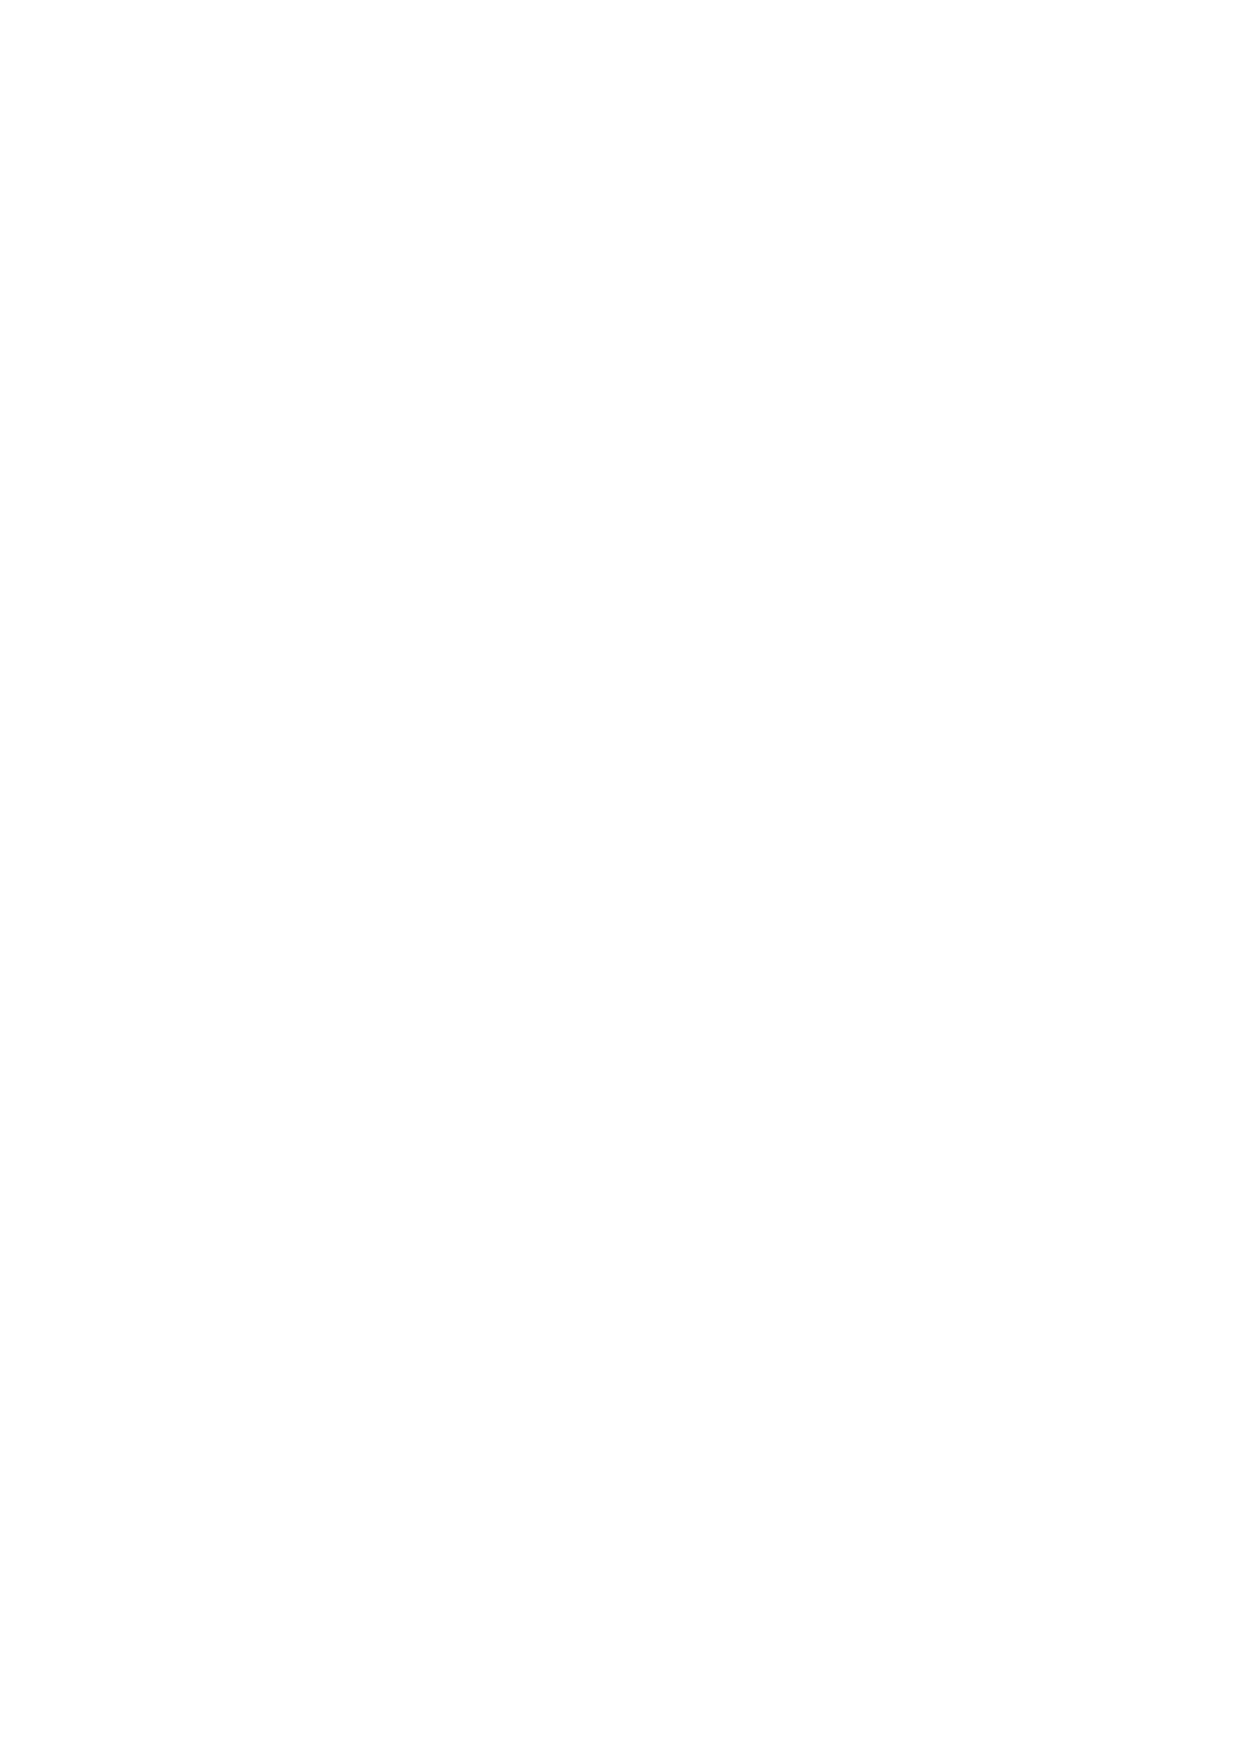
\includegraphics[width=\columnwidth]{./figs/ch3_angle_bisector}
		%\vspace*{-10cm}
		\resizebox{\columnwidth}{!}{\input{./figs/ang_bisect.tex}}
	\end{center}
	\caption{Tangent and incircle.}
	\label{fig:ang_bisect}	
\end{figure}


\item Show that $OD \perp BC$.
%\begin{figure}[!h]
%\centering
%\resizebox {\columnwidth} {!} {
%\input{./figs/derivative.tex}
%}
%\caption{Notion of the derivative.}
%\label{fig:derivative}
%\end{figure}
\\
\solution Let $\vec{x}_1,\vec{x}_2$ be two points on the circle such that 
$x_1x_2 \parallel BC$. Then
%
\begin{align}
\norm{\vec{x}_1-\vec{O}}^2- 
\norm{\vec{x}_2-\vec{O}}^2 &= 0 
\\
\implies 
\brak{\vec{x}_1-\vec{x}_2}^T\brak{\frac{\vec{x}_1+\vec{x}_2}{2}-\vec{O}} &= 
0 
\\
\implies 
\brak{\vec{B}-\vec{C}}^T\brak{\frac{\vec{x}_1+\vec{x}_2}{2}-\vec{O}} &= 
0 
%\label{eq:circle_bisect}
\end{align}
%
For $\vec{x}_1=\vec{x}_2=\vec{D}$, $x_1x_2$ merges into $BC$ and the above 
equation becomes 
%
\begin{align}
\brak{\vec{B}-\vec{C}}^T\brak{\vec{D}-\vec{O}} = 
0 
\implies OD \perp BC
%\label{eq:circle_bisect}
\end{align}
%
\item Give an alternative proof for the above.
\\
\solution Let 
\begin{align}
\vec{B} & = \mbf{0}
\\
\vec{D} &= \lambda \vec{m}
\end{align}
Then
\begin{align}
\norm{\vec{D} - \vec{O}}^2 = r^2 &
\\
\implies \lambda^2\norm{\vec{m}}^2 - 2\lambda\vec{m}^T\vec{O} + \norm{\vec{O}}^2 &= r^2 
\end{align}
Since the above equation has a single root,
\begin{align}
\lambda = \frac{\vec{m}^T\vec{O}}{\norm{\vec{m}}^2}
\label{eq:incircle_lam}
\end{align}
%
Thus, 
\begin{align}
\brak{\vec{D} - \vec{B}}^T\brak{\vec{D} - \vec{O}}
&= \brak{\lambda\vec{m}}^T
\brak{\lambda\vec{m}-\vec{O}}
\\
&=\lambda^2\norm{\vec{m}}^2-\lambda\vec{m}^T\vec{O}
\\
&= \mbf{O} \text{ (from \ref{eq:incircle_lam})}.
\\
\implies & OD \perp BC
\end{align}
\item Find the equation of the tangent at $\vec{D}$.
\\
\solution The equation of the tangent is given by 
\begin{align}
\brak{\vec{O}-\vec{D}}^T\brak{\vec{x}-\vec{D}}=0
%\label{eq:circle_bisect}
\end{align}
%
\item Show that the angle in a semi-circle is a right angle.
\begin{figure}[!h]
\centering
\resizebox {\columnwidth} {!} {
\input{./figs/semi_circle.tex}
}
\caption{Angle in a semi-circle.}
\label{fig:ch2_line}
\end{figure}
\\
\solution Let 
\begin{align}
\vec{O} = 0
\end{align}
From the given information,
\begin{align}
\label{eq:semi_circ_pt}
\norm{\vec{A}}^2 = \norm{\vec{B}}^2 = \norm{\vec{C}}^2 = r^2
\\
\norm{\vec{B}-\vec{C}}^2 =  \brak{2r}^2
\\
\vec{B} + \vec{C} = 0
\label{eq:semcirc_mid}
\end{align}
%
where $r$ is the radius of the circle. Thus,
\begin{multline}
\norm{\vec{A}-\vec{B}}^2 + \norm{\vec{A}-\vec{C}}^2 = 
2\norm{\vec{A}}^2 + \norm{\vec{B}}^2 + \norm{\vec{C}}^2
\\
-2\vec{A}^T\brak{\vec{B}+\vec{C}}
%\\
%\norm{\vec{B}-\vec{C}}^2 =  \brak{2r}^2
%\\
%\vec{B} + \vec{C} = 0
\end{multline}
From \eqref{eq:semcirc_mid} and \eqref{eq:semi_circ_pt},
\begin{multline}
\norm{\vec{A}-\vec{B}}^2 + \norm{\vec{A}-\vec{C}}^2 = 4r^2 = \norm{\vec{B}-\vec{C}}^2 
%\\
%\norm{\vec{B}-\vec{C}}^2 =  \brak{2r}^2
%\\
%\vec{B} + \vec{C} = 0
\end{multline}
Thus, using Baudhayana's theorem, $\triangle ABC$ is right angled.
\item 	Show that $PA.PB = PC^2$, where $PC$ is the tangent to the circle in Fig. \ref{fig:tangent_secant}.

	\begin{figure}[!hb]
		\begin{center}
			
			%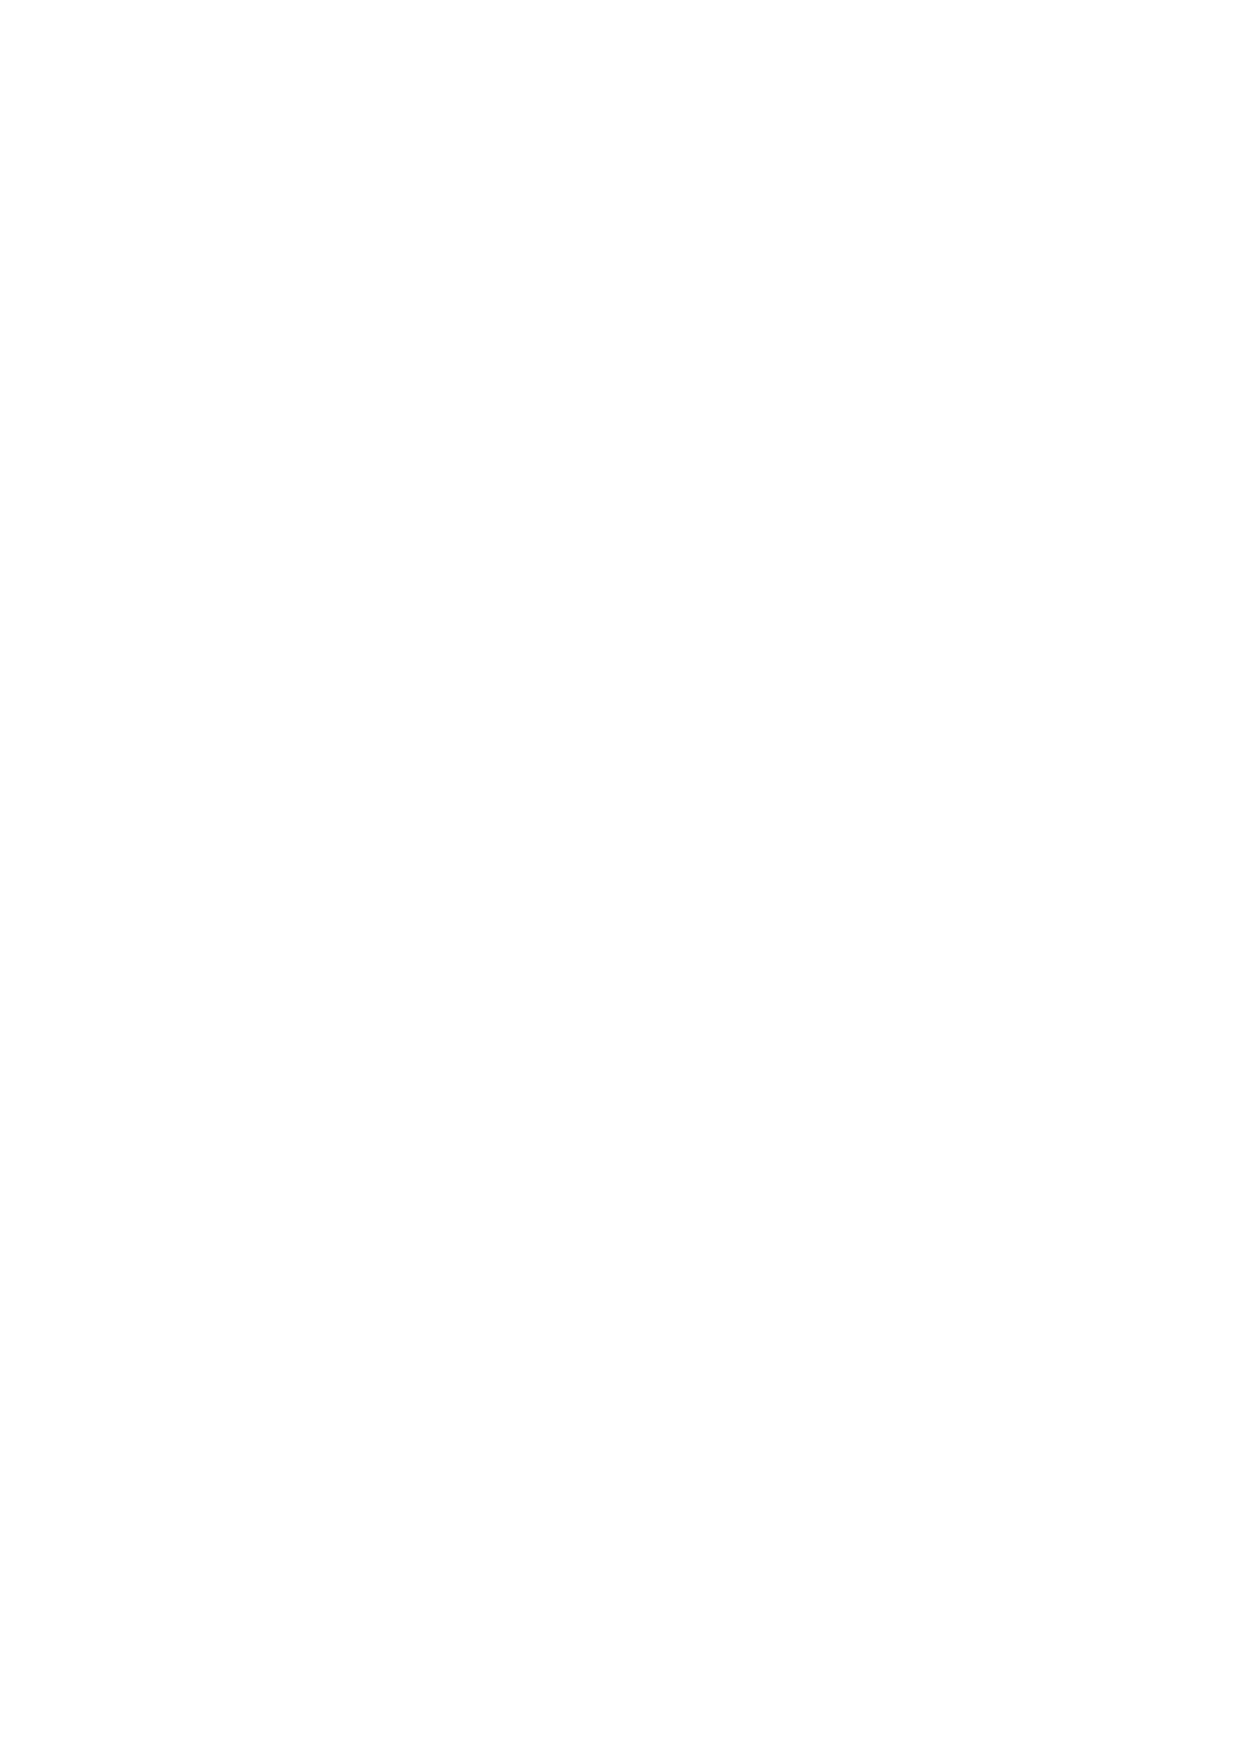
\includegraphics[width=\columnwidth]{./figs/ch4_tangent_prod}
			%\vspace*{-10cm}
			\resizebox{\columnwidth}{!}{\input{./figs/tangent_secant.tex}}
		\end{center}
		\caption{$PA.PB = PC^2$.}
		\label{fig:tangent_secant}	
	\end{figure}
\solution Let $\vec{P} = \mbf{0}$.  Then, we have the following equations
\begin{align}
\label{eq:tan_sec_AB}
PA.PB &= \lambda \norm{\vec{A}}^2 \quad \because (\vec{B} = \lambda \vec{A})
\\
\norm{\vec{A}-\vec{O}}^2 &= \norm{\vec{B}-\vec{O}}^2 = \norm{\vec{C}-\vec{O}}^2 = r^2
\\
\norm{\vec{O}}^2-\norm{\vec{C}}^2 &=  r^2 \quad \triangle PCO\text{ is 
right angled}
\label{eq:tan_sec_boudh}
\end{align}
$\because$
\begin{align}
%\label{eq:tan_sec_AB}
%PA.PB &= \lambda \norm{\vec{A}}^2 \quad \because (\vec{B} = \lambda 
%\vec{A})
%\\
\norm{\vec{B}-\vec{O}}^2-\norm{\vec{A}-\vec{O}}^2   &=0,
\\
\brak{\lambda^2-1}\norm{\vec{A}}^2 - 2 \brak{\lambda-1}\vec{A}^T\vec{O} &= 
0
\\
\implies PA.PB = \lambda\norm{\vec{A}}^2 =  2 
\vec{A}^T\vec{O}-\norm{\vec{A}}^2 &
%\norm{\vec{C}-\vec{O}}^2 = r^2
%\\
%\norm{\vec{O}}^2-\norm{\vec{C}}^2 &=  r^2 \quad \triangle PCO\text{ is 
%right angled}
%\label{eq:tan_sec_boudh}
\label{eq:tan_sec_first}
\end{align}
after substituting from \eqref{eq:tan_sec_AB} and simplifying. From 
\eqref{eq:tan_sec_boudh},
\begin{align}
\norm{\vec{A}-\vec{O}}^2 = \norm{\vec{O}}^2-\norm{\vec{C}}^2  &= r^2
\\
\implies 2 \vec{A}^T\vec{O}-\norm{\vec{A}}^2   = \norm{\vec{C}}^2 = PC^2&
\label{eq:tan_sec_second}
\end{align}
From \eqref{eq:tan_sec_first} and \eqref{eq:tan_sec_second},
\begin{align}
PA.PB = PC^2
\end{align}

\item In Fig. \ref{fig:chords} show that $PA.PB = PC.PD$.
\begin{figure}[!ht]
	\begin{center}
		
		%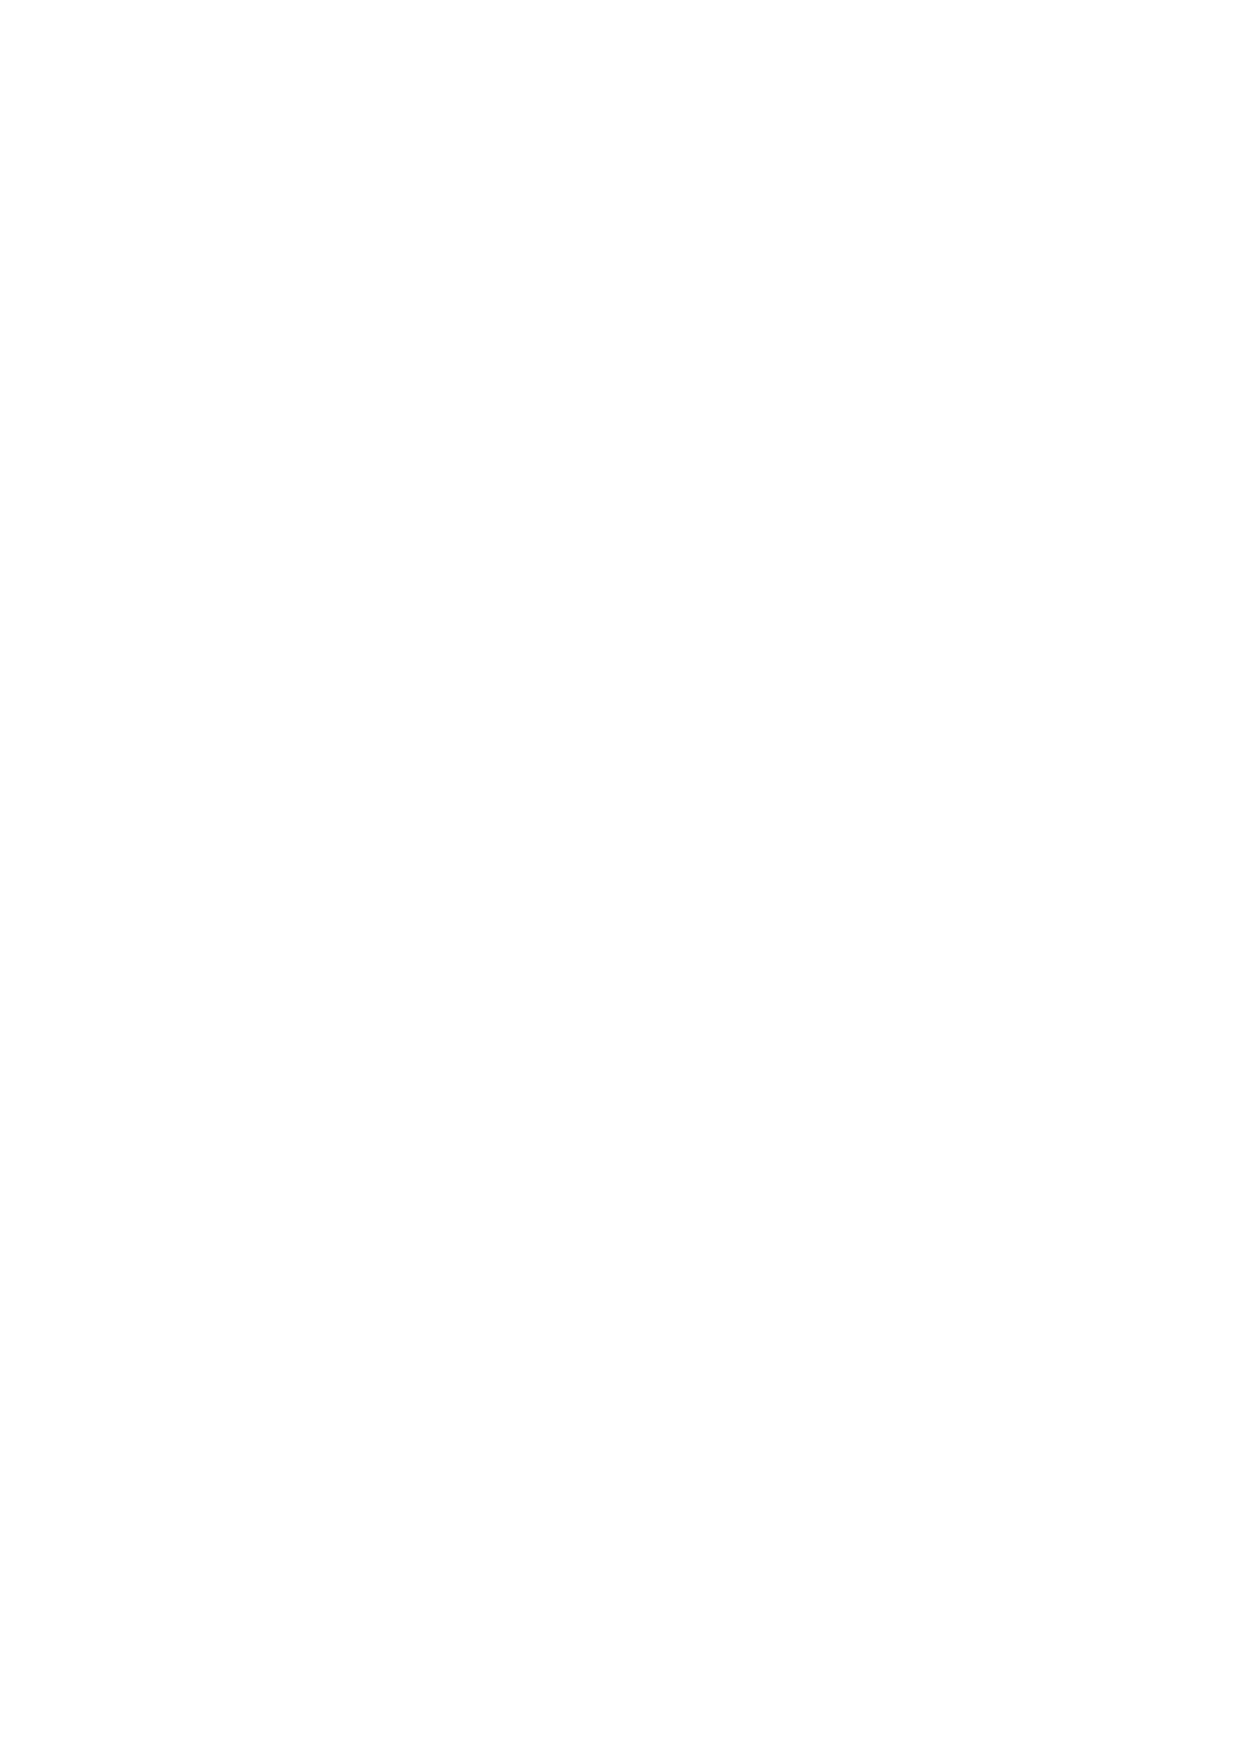
\includegraphics[width=\columnwidth]{./figs/ch3_angle_bisector}
		%\vspace*{-10cm}
		\resizebox{\columnwidth}{!}{\input{./figs/chords.tex}}
	\end{center}
	\caption{Chords of a circle}
	\label{fig:chords}	
\end{figure}
\\
\solution Let $\vec{P} = \mbf{0}$.  We then have the following equations
\begin{align}
\begin{split}
\vec{B} &= k_1 \vec{A}, k_1 = \frac{PB}{PA}
\\
\vec{D} &= k_2 \vec{C}, k_2 = \frac{PD}{PC}
\end{split}
\label{eq:chords_ratio}
\\
\begin{split}
\norm{\vec{A}-\vec{O}}^2 &= \norm{\vec{B}-\vec{O}}^2 
\\
= \norm{\vec{C}-\vec{O}}^2 &= \norm{\vec{D}-\vec{O}}^2 = r^2
\end{split}
\label{eq:chords_points}
\end{align}
%
where $r$ is the radius of the circle and $\vec{O}$ is the centre. From \eqref{eq:chords_points},
\begin{align}
&\norm{\vec{A}-\vec{O}}^2 = \norm{\vec{B}-\vec{O}}^2
\\
\implies &\norm{\vec{A}-\vec{O}}^2 = \norm{k\vec{A}-\vec{O}}^2 \quad(\text{from \eqref{eq:chords_ratio}})
\end{align}
%
which can be simplified to obtain
\begin{align}
k_1\norm{\vec{A}}^2 = 2\vec{A}^T\vec{O}-\norm{\vec{A}}^2
\label{eq:chords_Anorm}
\end{align}
Similarly,
\begin{align}
k_2\norm{\vec{C}}^2 = 2\vec{C}^T\vec{O}-\norm{\vec{C}}^2
\label{eq:chords_Cnorm}
\end{align}
%
From \eqref{eq:chords_points}, we also obtain
\begin{align}
\norm{\vec{A}-\vec{O}}^2 
= \norm{\vec{C}-\vec{O}}^2 
\\
\implies 2\vec{A}^T\vec{O}-\norm{\vec{A}}^2 = 2\vec{C}^T\vec{O}-\norm{\vec{C}}^2
\label{eq:chords_ACnorm}
\end{align}
%
after simplification. Using this result in \eqref{eq:chords_Anorm} and \eqref{eq:chords_Cnorm},
\begin{align}
k_1\norm{\vec{A}}^2 = k_2\norm{\vec{C}}^2
\\
\implies \norm{\vec{A}}\, \norm{\vec{B}}=\norm{\vec{C}}\,\norm{\vec{D}}
\end{align}
which completes the proof.

\item (Pole and Polar:) The polar of a point $\vec{x}$ with respect to the curve
\begin{align}
\label{eq:quad_form_polar}
\vec{x}^T\vec{V}\vec{x}+2\vec{u}^T\vec{x}+f=0
\end{align}
is the line
\begin{align}
\label{eq:polar}
\vec{n}^T\vec{x} = c
\end{align}
%
where
\begin{align}
\myvec{\vec{n}^T\\ - c}=
\myvec{
\vec{V}&\vec{u}
\\
\vec{u}^T&f
}
\myvec{\vec{x}\\1}
\end{align}
%
The pole of the line  in \eqref{eq:polar} is obtained as $\frac{1}{x_3}\myvec{x_1\\x_2}$, where
\begin{align}
\myvec{x_1 \\ x_2\\x_3}
=\myvec{
\vec{V}&\vec{u}
\\
\vec{u}^T&f
}^{-1}
\myvec{\vec{n}^T\\ - c}
\end{align}
\item $\vec{x}_1$ and $\vec{x}_2$ are said to be conjugate points for \eqref{eq:quad_form_polar} if $\vec{x}_2$ lies on the polar of $\vec{x}_1$ and vice-versa.  A similar definition holds for conjugate lines as well.

\end{enumerate}


